In this section, we describe the move execution layer. This layer is responsible for one of the key functionalities of our project which is the UR5 Robotic Arm's movement, which allows for the checkers game to take place between the user and the co-bot. The move execution layer is made up of three subsystems, the UR5 Robot Arm itself, the electromagnetic gripper, as well as an Arduino.

\subsection{UR5 Robot Arm}
\begin{figure}[h!]
	\centering
 	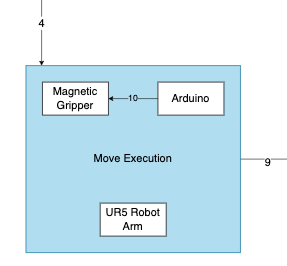
\includegraphics[width=0.60\textwidth]{images/move_execution.png}
 \caption{Move execution layer subsystems diagram}
\end{figure}

\subsubsection{Assumptions}
Here our biggest assumption is the fact that the UR5 arm has already been connected to the software functionality and therefore can be programmed to make specific moves.

\subsubsection{Responsibilities}
The UR5 co-bot arm must be able to follow the instructions as asked by the software in order to hover over the correct location on the checker board. The robot must be able to move to fixed locations as predetermined by ROS and our custom software in order to not only move to specified pieces on the board but also to the collection box, and a waiting position.

\subsubsection{Subsystem Interfaces}
\begin {table}[H]
\caption {UR5 Robot Arm interfaces} 
\begin{center}
    \begin{tabular}{ | p{1cm} | p{6cm} | p{3cm} | p{3cm} |}
    \hline
    ID & Description & Inputs & Outputs \\ \hline
    \#4 & Receive input from computer/software & \pbox{3cm}{Location of next move} & \pbox{3cm}{UR5 Arm will move to expected location}  \\ 
    \hline
    \end{tabular}
\end{center}
\end{table}

\subsection{Arduino}
\subsubsection{Assumptions}
N/A

\subsubsection{Responsibilities}
The Arduino system has the primary responsibility of being the micro-controller of our magnetic gripper. We will be integrating the Arduino into our software so that we can have the ability to turn our electromagnet on and off whenever we are moving our checkers pieces around.

\subsubsection{Subsystem Interfaces}
\begin {table}[H]
\caption {Arduino interfaces} 
\begin{center}
    \begin{tabular}{ | p{1cm} | p{6cm} | p{3cm} | p{3cm} |}
    \hline
    ID & Description & Inputs & Outputs \\ \hline
    \#4 & Receive input from computer/software & \pbox{3cm}{Signal indicating on/off} & \pbox{3cm}{Arduino will store on/off signal to send to magnetic gripper}  \\ \hline
    \#10 & Send signal to  magnetic gripper & \pbox{3cm}{Stored on/off signal in Arduino} & \pbox{3cm}{Send on/offsignal to magnetic gripper}  \\ 
    \hline
    \end{tabular}
\end{center}
\end{table}

\subsection{Magnetic Gripper}
\subsubsection{Assumptions}
We will assume that the magnetic gripper has been attached to the "hand" or tip of the UR5 Robot Arm, via a base that has been 3D printed.

\subsubsection{Responsibilities}
The Magnetic Gripper allows for game play interaction to take place as it will be the component that physically picks up and releases each individual checkers piece throughout the game.

\subsubsection{Subsystem Interfaces}
\begin {table}[H]
\caption {Magnetic Gripper interfaces}
\begin{center}
    \begin{tabular}{ | p{1cm} | p{6cm} | p{3cm} | p{3cm} |}
    \hline
    ID & Description & Inputs & Outputs \\ \hline
    \#10 & Receive signal from Arduino & \pbox{3cm}{On/off signal from Arduino} & \pbox{3cm}{Magnetic gripper will turn on/off accordingly}  \\ 
    \hline
    \end{tabular}
\end{center}
\end{table}

